\begin{frame}
\frametitle{Intel 8254}
\begin{itemize}
  \item Intel 8254 (aka PIT) - интервальный таймер, т. е. устройство
  генерирующее сигналы с заданной частотой;
  \begin{itemize}
    \item обычно PIT подключен к 0 входу Master PIC;
    \item у PIT есть 3 выхода, из которых к Master PIC подключен только 0-ой.
  \end{itemize}
  \item Частота работы PIT 1193180 Гц
  \begin{itemize}
    \item задав "коэффициент деления" можно получить меньшую частоту генерации
    сигналов;
    \item коэффциент деления k, значит, что на выход попадает только каждый k-ый
    сигнал.
  \end{itemize}
  \item PIT имеет внутренний счетчик
  \begin{itemize}
    \item мы можем задать начальное знаение для счетчика, и он будет уменьшаться
    на каждый сигнал пока не дойдет до 0;
    \item что произойдет дальше зависит от режима работы.
  \end{itemize}
\end{itemize}
\end{frame}

\begin{frame}
\frametitle{Режимы работы PIT}
\begin{itemize}
  \item One Shot (mode 0)
  \begin{itemize}
    \item задаем начальное значение счетчика, по достижении 0 генерируется
    прерывание, на этом работа останавливается.
  \end{itemize}
  \item Rate Generator (mode 2)
  \begin{itemize}
    \item по достижении 0 генерируется прерывание, счтечик перезагружается и
    отсчет повторяется заново.
  \end{itemize}
  \item Есть и другие режимы работы (но нам они не особо интересны):
  \begin{itemize}
    \item Square Wave Generator (mode 3);
    \item Softaware Triggered Strobe (mode 4);
    \item и другие...
  \end{itemize}
\end{itemize}
\end{frame}

\begin{frame}
\frametitle{Программирование PIT}
\begin{itemize}
  \item Прогруммирование PIT осуществляется через два порта ввода/вывода:
  \begin{itemize}
    \item Control Port \emph{0x43} - "команда" и выбор канала (в нашем случае
    канал всегда 0);
    \item Data Port \emph{0x40} - данные команды (у кадого канала свой Data Port
    \emph{0x40} используется для 0-ого).
  \end{itemize}
\end{itemize}
\end{frame}

\begin{frame}
\frametitle{Формат команды PIT}
\begin{center}
  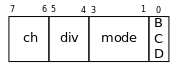
\includegraphics[width=0.4\textwidth]{pit_cmd.png}
\end{center}
\begin{itemize}
  \item BCD - формат представления чисел (вам точно не нужна 1 в этом бите);
  \item mode - режим работы;
  \item div - какие байты делителя вы хотите задать (делитель 16-битное число):
  \begin{itemize}
    \item 1 - хотим записать только младший байт;
    \item 2 - хотим записать только старший байт;
    \item 3 - хотим записать оба байта;
  \end{itemize}
  \item ch - канал, нам нужен 0.
\end{itemize}
\end{frame}

\begin{frame}
\frametitle{Задание коэффициента деления}
\begin{itemize}
  \item Если в команде поле div не 0, то PIT будет ожидать записи коэффициента
  деления в Data Port;
  \begin{itemize}
    \item если в поле div установлен только один бит, то нужно просто записать
    соответсвующий байт в Data Port;
    \item если в поле div установлены оба бита, то сначала нужно записать
    младший байт, а затем старший байт.
  \end{itemize}
\end{itemize}
\end{frame}
